\documentclass[a4paper]{article}
\usepackage[utf8x]{inputenc}
\usepackage[T1,T2A]{fontenc}
\usepackage[russian]{babel}
\usepackage{hyperref}
\usepackage{indentfirst}
\usepackage{listings}
\usepackage{color}
\usepackage{here}
\usepackage{array}
\usepackage{multirow}
\usepackage{graphicx}

\usepackage{caption}
\renewcommand{\lstlistingname}{Программа} % заголовок листингов кода

\usepackage{listings}
\lstset{ %
extendedchars=\true,
keepspaces=true,
language=bash,					% choose the language of the code
basicstyle=\footnotesize,		% the size of the fonts that are used for the code
numbers=left,					% where to put the line-numbers
numberstyle=\footnotesize,		% the size of the fonts that are used for the line-numbers
stepnumber=1,					% the step between two line-numbers. If it is 1 each line will be numbered
numbersep=5pt,					% how far the line-numbers are from the code
backgroundcolor=\color{white},	% choose the background color. You must add \usepackage{color}
showspaces=false				% show spaces adding particular underscores
showstringspaces=false,			% underline spaces within strings
showtabs=false,					% show tabs within strings adding particular underscores
frame=single,           		% adds a frame around the code
tabsize=2,						% sets default tabsize to 2 spaces
captionpos=b,					% sets the caption-position to bottom
breaklines=true,				% sets automatic line breaking
breakatwhitespace=false,		% sets if automatic breaks should only happen at whitespace
escapeinside={\%*}{*)},			% if you want to add a comment within your code
postbreak=\raisebox{0ex}[0ex][0ex]{\ensuremath{\color{red}\hookrightarrow\space}}
}

\usepackage[left=2cm,right=2cm,
top=2cm,bottom=2cm,bindingoffset=0cm]{geometry}


\begin{document}	% начало документа
	
	\begin{titlepage}	% начало титульной страницы

	\begin{center}		% выравнивание по центру

		\large Санкт-Петербургский Политехнический Университет Петра Великого\\
		\large Институт компьютерных наук и технологий \\
		\large Кафедра компьютерных систем и программных технологий\\[6cm]
		% название института, затем отступ 6см
		
		\huge Алгоритмы и структуры данных\\[0.5cm] % название работы, затем отступ 0,5см
		\large Отчет по курсовой работе\\[0.1cm]
		\large Игра змейка\\[5cm]

	\end{center}


	\begin{flushright} % выравнивание по правому краю
		\begin{minipage}{0.25\textwidth} % врезка в половину ширины текста
			\begin{flushleft} % выровнять её содержимое по левому краю

				\large\textbf{Работу выполнил:}\\
				\large Курякин Д. А.\\
				\large {Группа:} 23501/4\\
				
				\large \textbf{Преподаватель:}\\
				\large Вылегжанина К.Д.

			\end{flushleft}
		\end{minipage}
	\end{flushright}
	
	\vfill % заполнить всё доступное ниже пространство

	\begin{center}
	\large Санкт-Петербург\\
	\large \the\year % вывести дату
	\end{center} % закончить выравнивание по центру

\thispagestyle{empty} % не нумеровать страницу
\end{titlepage} % конец титульной страницы

\vfill % заполнить всё доступное ниже пространство

	
	
	% Содержание
	\tableofcontents
	\newpage
	
	
	
	\section{Игра Змейка}
	
	\subsection{Игровые принадлежности}
	
	Змейка — компьютерная игра, возникшая в середине или в конце 1970-х.
	
	Игрок управляет длинным, тонким существом, напоминающим змею, которое ползает по плоскости ограниченной стенками, собирая еду, избегая столкновения с собственным хвостом и краями игрового поля. Каждый раз, когда змея съедает кусок пищи, она становится длиннее, что постепенно усложняет игру. Игрок управляет направлением движения головы змеи: вверх, вниз, влево, вправо, а хвост змеи движется следом. Игрок не может остановить движение змеи.
	
	\subsection{Порядок использования}
	
	После начала игры появляется еда(яблоко). Пользователь направлет голову змейки чтобы съесть яблоко. После съедения яблока змейка увеличивается на одно деление. Затем яблоко появляется в любом месте на карте.
	
	\section{Проектирование приложения}
	
	\subsection{Концепция приложения} 
	
	В ходе проектирования было разработана концепция продукта.
	Созданное приложение должно предполагать возможность: управления змейкой с помощью свейпа по экрану, появления яблок на карте, съедения яблок, увеличения размера змейки. 
	
	\subsection{Минимально работоспособный продукт}
	
	Минимальном работоспособным продуктом было признано приложение, позволяющие производить игру(управлять змейкой, съедать яблоко, увеличивать длину после съедания). 
	
	\subsection{Прецеденты использования}
	
	На основе разработанной концепции была составлена UML диаграмма прецедентов использования (рис.\ref{pic:use_case}).
	
	\begin{figure}[H]
		\begin{center}
		\begin{minipage}[h]{0.49\linewidth}
			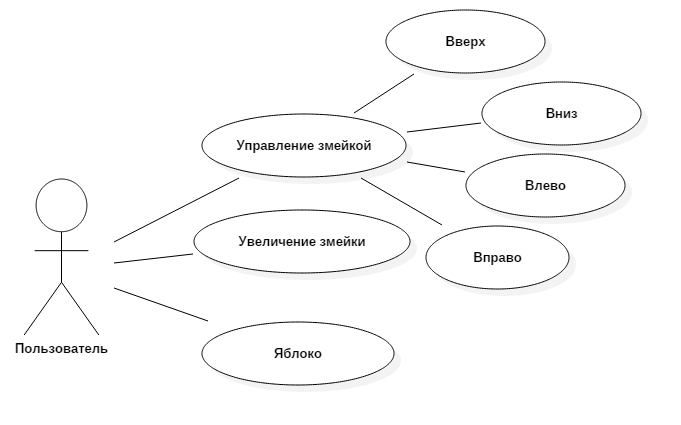
\includegraphics[width=1\textwidth]{../image/UseCases.png}
			\caption{Диаграмма прецедентов использования}
			\label{pic:use_case}
		\end{minipage}
	\end{center}
	\end{figure}
	
	\subsection{Основные компоненты приложения}
	
	На основе анализа концепции и выделенных прецедентов использования было принято решение выделить два основных компонента, которые будут входить в состав продукта:
	
	\begin{enumerate}
		\item Библиотека
		
		Включает в себя игровую модель и реализует игровые механизмы. В ядре должно быть обеспечено регулярное обновление модели в ответ на действие пользователя. Кроме того, должна быть реализована обработка исключительных ситуаций, включающие в себя ошибки игрока, попытки выполнить запрещенные действия и прочее.
		
		\item Графическое приложение 
		
		Графически визуализирует игровую модель, предоставляет пользователю графический интерфейс для взаимодействия с ней и выполнения остальный действий предусмотренных в реализации библиотеки. 
	\end{enumerate}
	
	\subsection{Используемые инструменты}
	
	Разработка в основном велась с использованием средств стандартной библиотеки Java в среде Android Studio. Для создания графического интерфейса применялась библиотеки из Android Studio. 
	
	\subsubsection{Android Studio}
	
	Android Studio — это интегрированная среда разработки (IDE) для работы с платформой Android.
	
	\subsection{Выводы}
	Таким образом, была разработана концепция приложения, что позволило определить внешний вид продукта и выделить его основные компоненты.
	
	\section{Реализация приложения}
	
	\subsection{Среда разработки}
	
	\begin{itemize}
		\item Операционная система: Windows 10
		\item Интегрирование среда разработки: Android Studio 2.3
		\item Версия SDK: 26.0.2
	\end{itemize}
	
	\subsection{Реализация основных компонентов приложения}
	
	\subsubsection{Библиотека Core}
	
	Для реализации всех запланированных функциональностей было принято решение, создать два класса:
	
	\begin{enumerate}
		
		\item \textbf{Класс Coordinate}
		Данный класс представляет возможность управлять координатами обьекта. Конструктор класса \textbf{Coordinate} получает на вход координаты объекта \textbf{X} и \textbf{Y}. С помошью методов \textbf{setX} и \textbf{setY} предоставляется возможность изменять координаты объектов. Методы \textbf{getX} и \textbf{getY} предоставляют возможность возвращать координаты обьекта. Метод \textbf{equals} возвращает значение boolean и представляет возможность ставнивать обьекты друг с другом.
		
		\item \textbf{Класс GameEngine}
		Данный класс отвечает работу игры в целом. 
		Метод \textbf{initGame} отвечает за инициализацию всех объектов игры. Класс \textbf{addSnake} добавляет змейку, \textbf{addWalls}  добавляет стены, \textbf{addApples} добавляет яблоки.
		Метод \textbf{Update} отвечает за обновление всех объектов игры. Используя класс \textbf{UpdateSnake} и перечисляемый тип Enum \textbf{Direction} метод \textbf{Update} обновляет змейку: направление (Noth, East, South, West), координаты всех частей змейки. Также с помощью перечисляемого типа Enum \textbf{GameState} метод \textbf{Update} осуществляет статусы игры (Ready, Running, Lost)
		Метод \textbf{getMap} создаёт карту используя перечисляемый тип Enum \textbf{TileType} (Nothing, Wall, SnakeHead, SnakeTail, Apple)
		
	\end{enumerate}
	
	\subsubsection{Графический интерфейс}
	
		Для создания графического интерфейса использовалась библиотеки Android Studio. 
		В Android Studio было создано Main Activity в котором с помощью класса \textbf{SnakeView} осуществляется отрисовка. Также к Main Activity был применён интерфейс \textbf{View.OnTouchListener} для считывания касаний экрана.
		
	\begin{enumerate}
		\item \textbf{Класс SnakeView}
		Класс наследуется от класса \textbf{View} и осуществляет отрисовку игры методом \textbf{onDraw}.
	\end{enumerate}
	
	\begin{figure}[H]
		\begin{minipage}[h]{0.33\linewidth}
			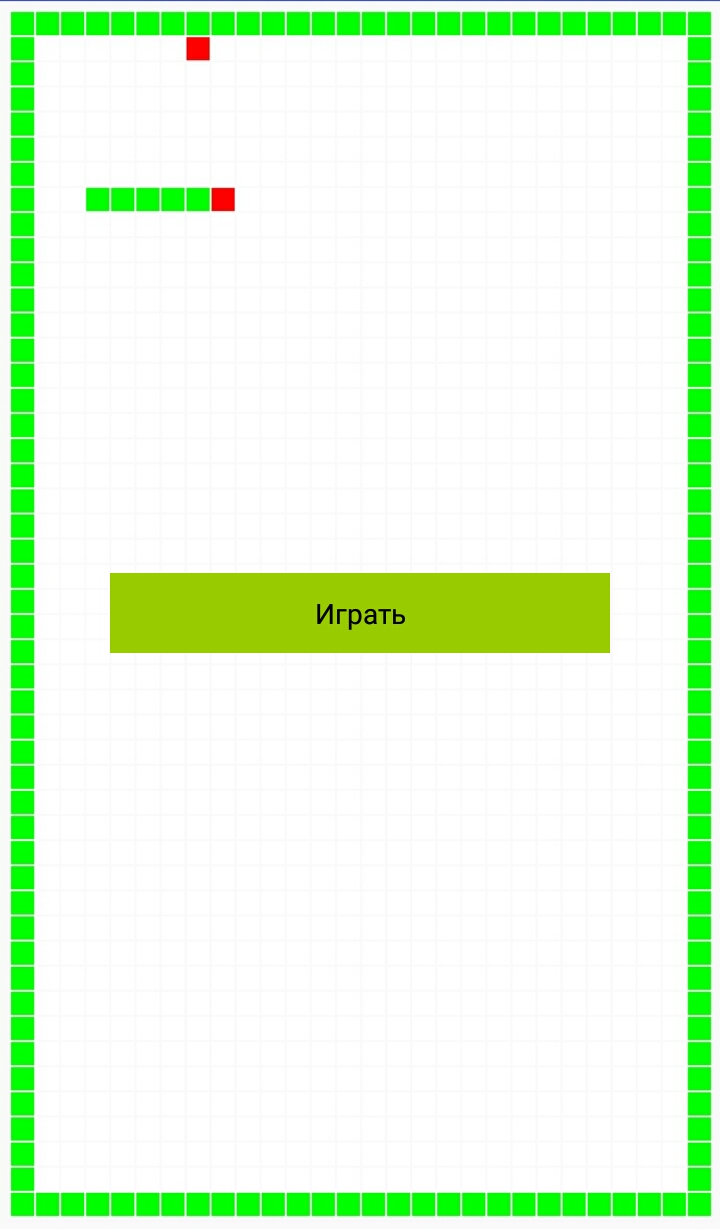
\includegraphics[width=1\textwidth]{../image/menu.png}
			\caption{Меню графического интерфейса}
			\label{pic:android_menu}
		\end{minipage}
		\hfill
		\begin{minipage}[h]{0.33\linewidth}
			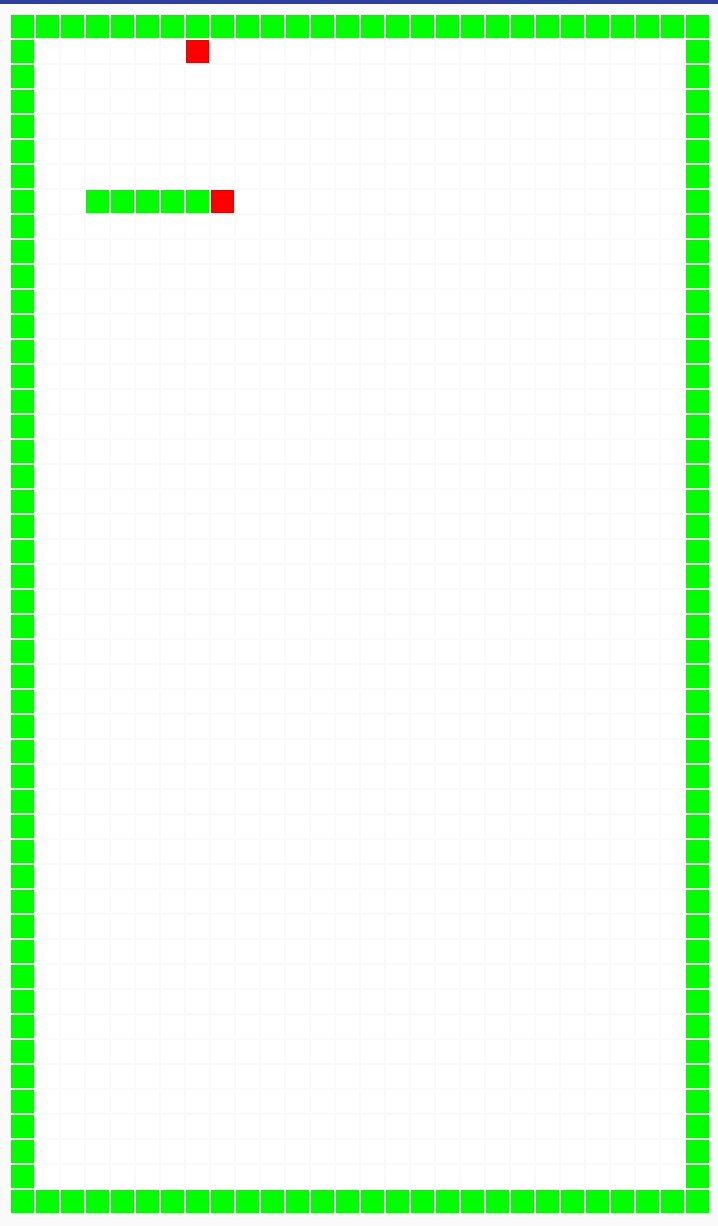
\includegraphics[width=1\textwidth]{../image/GameScreen1.png}
			\caption{Игровое окно графического интерфейса}
			\label{pic:android_screen1}
		\end{minipage}
	\end{figure} 
	
	На рисунках \ref{pic:android_menu}, \ref{pic:android_screen1} изображены основные окна графического интерфейса. 
	
	\subsection{Теститрование}
	
	В ходе разработки проекта регулярно проводилось ручное тестирование.
	
	Тестирование позволило обеспечить работоспособность продукта в ходе всего процесса разработки. 
	
	\subsection{Демонстрации}
	
	Во время создания приложения было проведено 1 демонстрации, на которых группой людей, представляющих собой потенциальных пользовоталей разработываемого приложения.
	
	\section{Выводы}
	
	В ходе работы были получены навыки необходимые для написания программ на языке программирования Java. Во-первых были изучены библиотеки Android Studio и особенности данной среды разработки. Во-вторых был получен опыт, связанный с процессом разработки программного продукта. 
	
	\section{Приложение 1}
	
	\subsection{Листинги}
	
	\lstinputlisting[]
	{H:/Snake/app/src/main/java/ru/kuryakin/snake/engine/Coordinate.java}
	
	\lstinputlisting[]
	{H:/Snake/app/src/main/java/ru/kuryakin/snake/engine/Direction.java}
	
	\lstinputlisting[]
	{H:/Snake/app/src/main/java/ru/kuryakin/snake/engine/GameEngine.java}
	
	\lstinputlisting[]
	{H:/Snake/app/src/main/java/ru/kuryakin/snake/engine/GameState.java}
	
	\lstinputlisting[]
	{H:/Snake/app/src/main/java/ru/kuryakin/snake/engine/TileType.java}
	
	\lstinputlisting[]
	{H:/Snake/app/src/main/java/ru/kuryakin/snake/views/SnakeView.java}
	
	\lstinputlisting[]
	{H:/Snake/app/src/main/java/ru/kuryakin/snake/MainActivity.java}
	
	\lstinputlisting[]
	{H:/Snake/app/src/main/res/layout/activity_main.xml}
	
\end{document}